\chapter{Imunidade Adaptativa e Vacinação}\label{ch:b3:adaptive-immunity}

Em 1796 um médico do interior raspou pus da ferida de varíola bovina de
uma ordenhadora para dentro do braço de um menino e, seis semanas
depois, inoculou-o com varíola; o menino não adoeceu. Em 1980 a
Organização Mundial da Saúde declarou a varíola --- que havia matado
trezentos milhões de pessoas no século XX --- erradicada da Terra, por
esse método. O sistema que Jenner recrutou sem saber que ele existia é
capaz de reconhecer qualquer molécula que nunca encontrou, escolher
entre cem bilhões de receptores diferentes os poucos que servem,
multiplicar um milhão de vezes numa semana as células que os carregam,
melhorar seu encaixe por mutação e seleção enquanto o faz, e lembrar o
resultado por toda a vida; ele também aprende a não atacar o corpo que
o fez, e suas falhas em aprender isso são as doenças autoimunes. Este
capítulo trata dos \omterm{def:b3:adaptive-immunity:lymphocytes}{linfócitos} e de como eles fabricam seus receptores,
de como uma resposta é montada e lembrada, de como a \omterm{def:b3:adaptive-immunity:tolerance}{tolerância} é
imposta e perdida, e da aritmética pela qual vacinar gente suficiente
protege quem não é vacinado.

\section{Linfócitos e seleção clonal}

\begin{definition}[Linfócitos e seus receptores]\label{def:b3:adaptive-immunity:lymphocytes}
\index{linfócito}\index{célula B}\index{célula T}\index{antígeno}\index{seleção clonal}\index{linfonodo}
A \emph{imunidade adaptativa} é sustentada pelos \emph{linfócitos}: as
\emph{células B}, que amadurecem na medula óssea e cujo receptor de
antígeno é um \emph{\omterm{def:b3:adaptive-immunity:antibody}{anticorpo}} ligado à membrana que mais tarde elas
secretam; e as \emph{células T}, que amadurecem no \omterm{def:b3:adaptive-immunity:tolerance}{timo} e cujo receptor
reconhece fragmentos de peptídeo exibidos na superfície de outras
células. Um \emph{antígeno} é tudo aquilo que um receptor liga; a parte
de fato contatada é um \emph{epítopo}. O fato fundador é a \emph{seleção
clonal} (Burnet, 1957): cada linfócito carrega receptores de uma só
especificidade, fixada antes de encontrar qualquer antígeno; o corpo
guarda um repertório de uns $10^{11}$ dessas células; um antígeno
seleciona os poucos cujos receptores servem e os leva a se dividir num
clone de células efetoras e de memória; e os linfócitos cujos
receptores servem às moléculas do próprio corpo são deletados ou
silenciados enquanto amadurecem. As células circulam continuamente
entre o sangue e os \emph{linfonodos}, o baço e o tecido linfoide das
mucosas, onde o antígeno trazido pelas \omterm{def:b3:innate-immunity:innate}{células dendríticas}
(\cref{ch:b3:innate-immunity}) é exibido, de modo que a rara célula
compatível --- uma em cem mil para um dado epítopo --- o encontra em um
ou dois dias.
\end{definition}

\begin{proof}[Evidência]
Nossal e Lederberg (1958) puseram \omterm{def:b3:adaptive-immunity:lymphocytes}{linfócitos} isolados de ratos
imunizados em microgotas e testaram o \omterm{def:b3:adaptive-immunity:antibody}{anticorpo} que cada um secretava:
toda célula fazia \omterm{def:b3:adaptive-immunity:antibody}{anticorpo} contra um dos dois \omterm{def:b3:adaptive-immunity:lymphocytes}{antígenos}, nunca contra
ambos. Burnet havia previsto isso no ano anterior. Tonegawa (1976)
comparou o DNA de um gene de \omterm{def:b3:adaptive-immunity:antibody}{anticorpo} em células embrionárias e num
\omterm{def:b3:cancer-biology:hallmarks}{tumor} secretor de \omterm{def:b3:adaptive-immunity:antibody}{anticorpo}: no embrião as partes variável e constante
ficavam distantes; no \omterm{def:b3:cancer-biology:hallmarks}{tumor} estavam unidas --- o gene tinha sido
cortado e emendado na célula somática, a primeira demonstração de um
genoma rearranjado de propósito.
\end{proof}

\section{Fabricar cem bilhões de receptores}

\begin{definition}[Estrutura do anticorpo e recombinação V(D)J]\label{def:b3:adaptive-immunity:antibody}
\index{anticorpo}\index{imunoglobulina}\index{recombinação V(D)J}\index{RAG}\index{diversidade juncional}\index{troca de classe}
Um \emph{anticorpo} (imunoglobulina) são duas cadeias pesadas idênticas
e duas cadeias leves idênticas, cada uma com um domínio \emph{variável}
na ponta e domínios \emph{constantes} atrás; cada um dos dois braços
liga um epítopo por três alças hipervariáveis do domínio variável
pesado e três do leve, e a haste (Fc) é o que os fagócitos, o
\omterm{def:b3:innate-immunity:complement}{complemento} e os mastócitos reconhecem. Cinco classes diferem na região
constante da cadeia pesada: a IgM, a primeira feita, um pentâmero que
ativa bem o \omterm{def:b3:innate-immunity:complement}{complemento}; a IgG, o cavalo de batalha do sangue e dos
tecidos, que atravessa a placenta; a IgA, um dímero secretado através
das superfícies mucosas para o intestino, as vias aéreas e o leite; a
IgE, presa aos mastócitos, contra vermes --- e a causa da alergia; e a
IgD. Os domínios variáveis não são codificados como tais. O lócus da
cadeia pesada guarda cerca de $40$ segmentos \emph{V} funcionais, $25$
\emph{D} e $6$ \emph{J}; uma \omterm{def:b3:adaptive-immunity:lymphocytes}{célula B} em desenvolvimento escolhe um de
cada e os une por \emph{recombinação V(D)J}: as enzimas RAG1 e RAG2
cortam em sequências-sinal de recombinação que flanqueiam os segmentos,
e as pontas são unidas pela maquinaria de \omterm{def:b3:dna-repair:dsb}{junção de extremidades não
homólogas} do \cref{ch:b3:dna-repair}, com nucleotídeos aparados e
acrescentados ao acaso (pela enzima TdT) em cada junção --- a
\emph{diversidade juncional}, que cai exatamente na terceira alça
hipervariável. As cadeias leves fazem o mesmo com V e J. Depois que a
resposta começa, o mesmo domínio variável é unido a uma região
constante diferente por um segundo rearranjo, a \emph{troca de classe},
que muda a função do anticorpo mas não sua especificidade.
\end{definition}

\begin{theorem}[O tamanho do repertório]\label{thm:b3:adaptive-immunity:repertoire}
\index{repertório!combinatório}
Com $V_{H} = 40$, $D = 25$, $J_{H} = 6$ segmentos pesados e cadeias
leves de dois loci com $(V_{\kappa}, J_{\kappa}) = (40, 5)$ e
$(V_{\lambda}, J_{\lambda}) = (30, 4)$, o número de combinações
pesada--leve distintas obtidas só pela escolha de segmentos é
\[
(40\times 25\times 6)\times(40\times 5 + 30\times 4) = 6000\times 320
= 1.9\times 10^{6}.
\]
A \omterm{def:b3:adaptive-immunity:antibody}{diversidade juncional} nas duas junções pesadas e na junção leve
multiplica isso por um fator da ordem de $10^{4}$--$10^{5}$, dando um
repertório potencial acima de $10^{10}$ a partir de menos de $200$
segmentos gênicos --- mais do que o número de \omterm{def:b3:adaptive-immunity:lymphocytes}{células B} de um corpo, de
modo que o repertório efetivo é uma amostra do possível. A \omterm{def:b3:adaptive-immunity:germinal-centre}{hipermutação
somática} durante a resposta (adiante) gera então variantes de cada
receptor selecionado.
\end{theorem}
\begin{proof}
Cada cadeia pesada é um V, um D e um J; cada cadeia leve, um V e um J de
um dos dois loci; qualquer pesada se emparelha com qualquer leve, de
modo que as contagens se multiplicam (princípio multiplicativo), e os
dois loci leves se somam. O fator juncional é o número de sequências
distintas que o aparo e a adição aleatórios podem produzir numa junção
--- ao menos algumas dezenas por junção --- elevado ao número de
junções; seu valor exato não é definido, mas três junções com $30$--$50$
desfechos cada dão de $3\times 10^{4}$ a $10^{5}$. A contagem para os
receptores das \omterm{def:b3:adaptive-immunity:lymphocytes}{células T}, com duas cadeias rearranjadas do mesmo modo e
uma contribuição juncional maior, é da mesma ordem.
\end{proof}

\begin{omfigure}
\begin{tikzpicture}[every node/.style={font=\scriptsize}, >=stealth]
  % antibody Y
  \begin{scope}[xshift=0cm]
    % heavy chains
    \draw[very thick, omDef] (0,0) -- (0,1.6) -- (-1.3,3.0); \draw[very thick, omDef] (0.35,0) -- (0.35,1.6) -- (1.65,3.0);
    % light chains
    \draw[very thick, omProp] (-0.45,1.55) -- (-1.75,2.95); \draw[very thick, omProp] (0.8,1.55) -- (2.1,2.95);
    \fill[omThm] (-1.55,3.0) circle (0.12); \fill[omThm] (1.9,3.0) circle (0.12);
    \node[above, align=center] at (-1.5,3.15) {domínios variáveis:\\sítio de ligação\\ao antígeno}; 
    \node[right, align=left] at (0.55,0.5) {haste Fc (constante):\\a classe decide a função};
    \node[left, omProp] at (-0.7,2.1) {leve}; \node[right, omDef] at (0.4,1.3) {pesada};
    \draw[omDef] (0.05,1.1) -- (0.3,1.1); \draw[omDef] (0.05,0.7) -- (0.3,0.7);
  \end{scope}
  % V(D)J locus
  \begin{scope}[xshift=4.2cm, yshift=2.4cm, xscale=0.86]
    \draw[very thick, gray] (0,0) -- (8.2,0);
    \foreach \x in {0.2,0.6,1.0,1.4} \draw[thick, fill=omDef!40] (\x,-0.15) rectangle (\x+0.3,0.15);
    \node[above] at (0.95,0.2) {segmentos V ($\sim 40$)}; \node[font=\tiny] at (1.95,0) {$\cdots$};
    \foreach \x in {2.5,2.8,3.1} \draw[thick, fill=omProp!50] (\x,-0.15) rectangle (\x+0.2,0.15);
    \node[above] at (2.9,0.2) {D ($25$)};
    \foreach \x in {3.8,4.1,4.4} \draw[thick, fill=omMeth!50] (\x,-0.15) rectangle (\x+0.2,0.15);
    \node[above] at (4.2,0.2) {J ($6$)};
    \foreach \x/\lab in {5.3/\mu,6.0/\delta,6.7/\gamma,7.4/\alpha} { \draw[thick, fill=gray!30] (\x,-0.15) rectangle (\x+0.5,0.15); \node[above] at (\x+0.25,0.2) {C$_{\lab}$}; }
    \draw[->, thick] (4.1,-0.4) -- (4.1,-1.1) node[midway, right, align=left, font=\tiny] {a RAG corta nas sequências-sinal;\\um V, um D e um J são unidos,\\a TdT acrescenta nucleotídeos ao acaso};
    % rearranged
    \draw[very thick, gray] (0,-1.5) -- (3.3,-1.5);
    \draw[thick, fill=omDef!40] (1.0,-1.65) rectangle (1.3,-1.35); \fill[omThm] (1.3,-1.65) rectangle (1.4,-1.35);
    \draw[thick, fill=omProp!50] (1.4,-1.65) rectangle (1.6,-1.35); \fill[omThm] (1.6,-1.65) rectangle (1.7,-1.35);
    \draw[thick, fill=omMeth!50] (1.7,-1.65) rectangle (1.9,-1.35);
    \draw[thick, fill=gray!30] (2.6,-1.65) rectangle (3.1,-1.35); \node[above] at (2.85,-1.3) {C$_{\mu}$};
    \node[below, align=center] at (1.45,-1.7) {VDJ unidos: o domínio variável,\\em vermelho: nucleotídeos juncionais};
    \node[right, align=left, font=\tiny] at (3.4,-2.0) {emendado a C$_{\mu}$: cadeia\\pesada de IgM; a troca de\\classe une depois o mesmo\\VDJ a C$_{\gamma}$ ou a C$_{\alpha}$};
  \end{scope}
\end{tikzpicture}

{\small À esquerda: um \omterm{def:b3:adaptive-immunity:antibody}{anticorpo} --- duas cadeias pesadas e duas leves,
os domínios variáveis nas pontas formando dois sítios de ligação, a
haste constante lida pelo resto do sistema imune. À direita: o lócus da
cadeia pesada antes e depois da \omterm{def:b3:adaptive-immunity:antibody}{recombinação V(D)J}, que escolhe um
segmento de cada tipo e acrescenta nucleotídeos ao acaso nas junções.}
\end{omfigure}

\begin{definition}[Receptores das células T e MHC]\label{def:b3:adaptive-immunity:mhc}
\index{receptor de células T}\index{complexo principal de histocompatibilidade}\index{apresentação de antígeno}\index{restrição pelo MHC}\index{HLA}
O \emph{receptor de \omterm{def:b3:adaptive-immunity:lymphocytes}{células T}} é uma molécula de duas cadeias
construída pela mesma recombinação, nunca secretada, e não liga
\omterm{def:b3:adaptive-immunity:lymphocytes}{antígeno} livre em solução: reconhece um peptídeo curto alojado na fenda
de uma molécula do \emph{complexo principal de histocompatibilidade}
(MHC) na superfície de outra célula. O \emph{MHC de classe~I}, em toda
célula nucleada, exibe peptídeos de oito a dez resíduos cortados pelo
proteassomo a partir das próprias proteínas citosólicas da célula ---
uma amostra do que a célula está fabricando, inclusive qualquer \omterm{def:b3:virology:virus}{vírus}
--- às \omterm{def:b3:adaptive-immunity:lymphocytes}{células T} \emph{CD8}, que matam a célula se o peptídeo for
estranho. O \emph{MHC de classe~II}, nas \omterm{def:b3:innate-immunity:innate}{células dendríticas}, nos
\omterm{def:b3:innate-immunity:innate}{macrófagos} e nas \omterm{def:b3:adaptive-immunity:lymphocytes}{células B}, exibe peptídeos de treze a vinte e cinco
resíduos de proteínas que a célula captou e digeriu em \omterm{def:b3:membrane-traffic:endocytosis}{endossomos}, às
\omterm{def:b3:adaptive-immunity:lymphocytes}{células T} \emph{CD4}, que respondem ajudando. Uma \omterm{def:b3:adaptive-immunity:lymphocytes}{célula T} é
\emph{restrita}: ela reconhece seu peptídeo apenas no alelo de MHC sobre
o qual foi selecionada. Os genes do MHC (\emph{HLA} nos humanos) são os
mais polimórficos do genoma, com milhares de alelos diferindo cada um
na fenda, de modo que cada pessoa exibe uma amostra diferente dos
peptídeos de cada proteína e nenhum patógeno consegue escapar da
apresentação em todo mundo --- e de modo que um órgão transplantado de
um doador incompatível é reconhecido como estranho por grande parte das
\omterm{def:b3:adaptive-immunity:lymphocytes}{células T} do receptor.
\end{definition}

\begin{proof}[Evidência]
Zinkernagel e Doherty (1974) infectaram camundongos de duas linhagens
consanguíneas com um \omterm{def:b3:virology:virus}{vírus} e testaram suas \omterm{def:b3:adaptive-immunity:response}{células T citotóxicas} sobre
células-alvo infectadas: as \omterm{def:b3:adaptive-immunity:lymphocytes}{células T} mataram células infectadas de sua
própria linhagem, mas não as da outra, embora o \omterm{def:b3:virology:virus}{vírus} fosse o mesmo. A
\omterm{def:b3:adaptive-immunity:lymphocytes}{célula T} via o \omterm{def:b3:virology:virus}{vírus} apenas junto com uma molécula de MHC própria --- a
\emph{\omterm{def:b3:adaptive-immunity:mhc}{restrição pelo MHC}} ---, o que foi explicado depois, quando a
estrutura cristalográfica de uma molécula de MHC (Bjorkman, 1987)
mostrou uma fenda com um peptídeo dentro, e se mostrou que o receptor
da \omterm{def:b3:adaptive-immunity:lymphocytes}{célula T} liga os dois ao mesmo tempo.
\end{proof}

\begin{omfigure}
\begin{tikzpicture}[every node/.style={font=\scriptsize}, >=stealth]
  % class I pathway
  \begin{scope}
    \draw[thick, omDef, fill=omDef!8] (0,0) rectangle (6.2,3.6); \node[anchor=north west] at (0.05,3.55) {qualquer célula nucleada};
    \node[draw, rounded corners, fill=omThm!20, font=\tiny, align=center] (v) at (1.4,2.6) {proteína viral ou própria\\no citosol};
    \node[draw, rounded corners, fill=gray!20, font=\tiny, align=center] (p) at (1.4,1.5) {proteassomo:\\peptídeos de 8--10};
    \node[draw, rounded corners, fill=omDef!25, font=\tiny, align=center] (er) at (4.6,1.5) {RE: carregados no\\MHC de classe I};
    \draw[->, thick] (v) -- (p); \draw[->, thick] (p) -- node[midway, above, font=\tiny] {TAP} (er);
    \draw[->, thick] (er) -- (4.6,3.55);
    \draw[thick, fill=omDef!40] (4.4,3.6) rectangle (4.8,4.1); \fill[omThm] (4.6,4.2) circle (0.09);
    \node[above, align=center] at (4.6,4.35) {peptídeo--MHC I\\visto pelas células T CD8: matam};
  \end{scope}
  % class II pathway
  \begin{scope}[xshift=7.2cm]
    \draw[thick, omProp, fill=omProp!8] (0,0) rectangle (6.2,3.6); \node[anchor=north west] at (0.05,3.55) {célula dendrítica, macrófago, célula B};
    \node[draw, rounded corners, fill=omThm!20, font=\tiny, align=center] (ex) at (1.4,2.6) {proteína captada\\para um endossomo};
    \node[draw, rounded corners, fill=gray!20, font=\tiny, align=center] (dig) at (1.4,1.5) {digerida:\\peptídeos de 13--25};
    \node[draw, rounded corners, fill=omProp!30, font=\tiny, align=center] (m2) at (4.6,1.5) {MHC de classe II\\carregado aqui};
    \draw[->, thick] (ex) -- (dig); \draw[->, thick] (dig) -- (m2);
    \draw[->, thick] (m2) -- (4.6,3.55);
    \draw[thick, fill=omProp!50] (4.4,3.6) rectangle (4.8,4.1); \fill[omThm] (4.6,4.2) circle (0.09);
    \node[above, align=center] at (4.6,4.35) {peptídeo--MHC II\\visto pelas células T CD4: ajudam};
  \end{scope}
\end{tikzpicture}

{\small As duas vias de apresentação. A classe~I mostra às \omterm{def:b3:adaptive-immunity:lymphocytes}{células T}
CD8 o que uma célula fabrica dentro de si; a classe~II mostra às
\omterm{def:b3:adaptive-immunity:lymphocytes}{células T} CD4 o que uma célula apresentadora de \omterm{def:b3:adaptive-immunity:lymphocytes}{antígeno} comeu. Uma
resposta citotóxica visa à primeira; uma resposta auxiliar, à segunda.}
\end{omfigure}

\section{A resposta}

\begin{definition}[Ativação, ajuda e morte]\label{def:b3:adaptive-immunity:response}
\index{célula T auxiliar}\index{célula T citotóxica}\index{coestimulação}\index{célula T reguladora}\index{plasmócito}\index{célula de memória}
Uma \omterm{def:b3:adaptive-immunity:lymphocytes}{célula T} virgem é ativada quando seu receptor liga peptídeo--MHC numa
\omterm{def:b3:innate-immunity:innate}{célula dendrítica} que também fornece coestimulação (\cref{ch:b3:innate-immunity});
ela então se divide a cada seis a oito horas por uma semana e se
diferencia. As \omterm{def:b3:adaptive-immunity:lymphocytes}{células T} \emph{auxiliares CD4} se diferenciam, conforme
as \omterm{def:b3:innate-immunity:inflammation}{citocinas} da \omterm{def:b3:innate-immunity:innate}{célula dendrítica}, em subgrupos: Th1, que ativam os
\omterm{def:b3:innate-immunity:innate}{macrófagos} a matar o que comeram (tuberculose); Th2, que impulsionam a
IgE e os eosinófilos contra os vermes; Th17, que recrutam \omterm{def:b3:innate-immunity:innate}{neutrófilos}
contra bactérias e fungos extracelulares; auxiliares foliculares, que
ajudam as \omterm{def:b3:adaptive-immunity:lymphocytes}{células B}; e as \omterm{def:b3:adaptive-immunity:lymphocytes}{células T} \emph{reguladoras}, que suprimem. As
\omterm{def:b3:adaptive-immunity:lymphocytes}{células T} \emph{citotóxicas CD8} matam as células que exibem seu
peptídeo na classe~I, pela perforina e pelas granzimas e pelo ligante de
Fas, disparando a \omterm{def:b3:cell-cycle-apoptosis:apoptosis}{apoptose} (\cref{ch:b3:cell-cycle-apoptosis}) --- a
defesa contra \omterm{def:b3:virology:virus}{vírus} e \omterm{def:b3:cancer-biology:hallmarks}{tumores}. Uma \omterm{def:b3:adaptive-immunity:lymphocytes}{célula B} é ativada pelo \omterm{def:b3:adaptive-immunity:lymphocytes}{antígeno} que
liga seu receptor, mais a ajuda de uma \omterm{def:b3:adaptive-immunity:lymphocytes}{célula T} auxiliar folicular que
reconhece peptídeos do mesmo \omterm{def:b3:adaptive-immunity:lymphocytes}{antígeno} na classe~II da \omterm{def:b3:adaptive-immunity:lymphocytes}{célula B}; ela
então se torna um \emph{plasmócito} que secreta milhares de \omterm{def:b3:adaptive-immunity:antibody}{anticorpos}
por segundo, por dias (de vida curta, no \omterm{def:b3:adaptive-immunity:lymphocytes}{linfonodo}) ou por anos (de vida
longa, na medula), ou entra num \omterm{def:b3:adaptive-immunity:germinal-centre}{centro germinativo}. As \omterm{def:b3:adaptive-immunity:lymphocytes}{células B} e T de
\emph{memória} --- de vida longa, mais numerosas que os precursores
virgens e mais rápidas a responder --- são o resíduo de toda resposta e
a base da vacinação.
\end{definition}

\begin{definition}[O centro germinativo]\label{def:b3:adaptive-immunity:germinal-centre}
\index{centro germinativo}\index{hipermutação somática}\index{maturação de afinidade}
Num \emph{centro germinativo}, estrutura que se forma num \omterm{def:b3:adaptive-immunity:lymphocytes}{linfonodo}
cerca de uma semana após o início de uma resposta, as \omterm{def:b3:adaptive-immunity:lymphocytes}{células B} ativadas
rodam um algoritmo evolutivo. Em sua zona escura elas se dividem a cada
seis horas e seus genes variáveis de \omterm{def:b3:adaptive-immunity:antibody}{anticorpo} são mutados pela enzima
AID a cerca de uma troca por mil pares de bases por divisão --- a
\emph{hipermutação somática}, um milhão de vezes a taxa genômica,
dirigida a uma quilobase. Na zona clara cada célula testa seu novo
receptor contra o \omterm{def:b3:adaptive-immunity:lymphocytes}{antígeno} retido nas \omterm{def:b3:innate-immunity:innate}{células dendríticas} foliculares e
compete pela ajuda das \omterm{def:b3:adaptive-immunity:lymphocytes}{células T}: as células que ligam melhor captam
mais \omterm{def:b3:adaptive-immunity:lymphocytes}{antígeno}, apresentam mais, recebem mais ajuda e voltam à zona
escura para se dividir de novo; as que ligam pior, ou perderam a
ligação, morrem por \omterm{def:b3:cell-cycle-apoptosis:apoptosis}{apoptose}. Ao longo de duas a três semanas de ciclos
a afinidade dos \omterm{def:b3:adaptive-immunity:antibody}{anticorpos} sobreviventes sobe de cem a mil vezes --- a
\emph{maturação de afinidade} --- e os vencedores saem como \omterm{def:b3:adaptive-immunity:response}{plasmócitos}
e \omterm{def:b3:adaptive-immunity:response}{células de memória}, tendo também trocado de classe. A resposta
secundária é mais rápida, maior e feita de \omterm{def:b3:adaptive-immunity:antibody}{anticorpo} melhor porque parte
dessa população selecionada, expandida e trocada de classe.
\end{definition}

\begin{omfigure}
\begin{tikzpicture}[every node/.style={font=\scriptsize}, >=stealth]
  \draw[thick, omDef, fill=omDef!12] (0,0) ellipse (2.7 and 1.7); \node[above, omDef!70!black] at (0,1.75) {zona escura};
  \draw[thick, omMeth!70!black, fill=omMeth!12] (6.2,0) ellipse (2.7 and 1.7); \node[above, omMeth!60!black] at (6.2,1.75) {zona clara};
  \node[align=center] at (0,0.3) {as células B se dividem a cada \qty{6}{h};\\a AID muta os genes do\\anticorpo: $10^{-3}$ por pb por divisão};
  \node[align=center] at (6.2,0.3) {testam o novo receptor\\no antígeno retido pelas\\células dendríticas foliculares;\\competem pela ajuda das células T};
  \draw[->, very thick, omProp] (2.4,0.7) .. controls (3.6,1.4) and (4.2,1.4) .. (3.7,0.7); \node[above, omProp] at (3.1,1.45) {saem os mutantes};
  \draw[->, very thick, omMeth!70!black] (3.7,-0.7) .. controls (4.2,-1.4) and (3.6,-1.4) .. (2.4,-0.7); \node[below, omMeth!70!black] at (3.1,-1.45) {voltam os vencedores, para dividir de novo};
  \draw[->, thick, omThm] (6.6,-1.6) -- (6.6,-2.3); \node[below, omThm, align=center] at (6.6,-2.3) {perdedores: apoptose\\(a maioria)};
  \draw[->, thick] (8.9,0) -- (9.5,0); \node[right, align=left] at (9.5,0) {após 2--3 semanas:\\plasmócitos (de vida longa,\\na medula) e células B\\de memória; afinidade\\$100$--$1000\times$ maior, trocada};
\end{tikzpicture}

{\small O \omterm{def:b3:adaptive-immunity:germinal-centre}{centro germinativo} como máquina evolutiva: mutação na zona
escura, seleção na zona clara e ciclagem entre as duas até que os
\omterm{def:b3:adaptive-immunity:antibody}{anticorpos} que saem liguem muito melhor do que os que entraram.}
\end{omfigure}

\begin{example}[Cinética de uma resposta]\label{ex:b3:adaptive-immunity:kinetics}
Cerca de uma \omterm{def:b3:adaptive-immunity:lymphocytes}{célula B} em $10^{5}$ liga um dado epítopo, de modo que as
$10^{11}$ \omterm{def:b3:adaptive-immunity:lymphocytes}{células B} de um corpo abrigam uns $10^{6}$ precursores, dos
quais talvez uma centena encontre o \omterm{def:b3:adaptive-immunity:lymphocytes}{antígeno} no \omterm{def:b3:adaptive-immunity:lymphocytes}{linfonodo} de drenagem.
Dividindo-se a cada oito horas, cem células viram $10^{2}\times 2^{21} \approx 2\times 10^{8}$ em uma semana. O \omterm{def:b3:adaptive-immunity:antibody}{anticorpo} aparece no soro
depois de quatro a seis dias, a IgM primeiro, atinge o pico em cerca de
duas semanas e declina com meia-vida de três semanas para a IgG à
medida que os \omterm{def:b3:adaptive-immunity:response}{plasmócitos} de vida curta morrem, estabilizando-se no
nível que os \omterm{def:b3:adaptive-immunity:response}{plasmócitos} de vida longa da medula mantêm por anos. Uma
segunda exposição parte de $10^{4}$--$10^{5}$ \omterm{def:b3:adaptive-immunity:response}{células de memória} de alta
afinidade já trocadas para IgG: o \omterm{def:b3:adaptive-immunity:antibody}{anticorpo} sobe em dois dias, de dez a
cem vezes mais alto, e neutraliza o patógeno antes que ele possa se
estabelecer --- que é o que uma \omterm{def:b3:adaptive-immunity:vaccine}{vacina} compra.
\end{example}

\begin{omfigure}
\begin{tikzpicture}
\begin{axis}[
  width=0.7\linewidth, height=5.6cm,
  axis x line=bottom, axis y line=left,
  xmin=0, xmax=70, ymin=1, ymax=10000, ymode=log,
  xlabel={dias}, ylabel={anticorpo sérico (relativo)},
  xlabel style={font=\small, at={(axis description cs:0.5,-0.12)}, anchor=north}, ylabel style={font=\small},
  tick label style={font=\small}, xtick={0,10,20,30,40,50,60,70},
  clip=false,
]
\addplot[very thick, omDef, domain=0:40, samples=60] {1 + 100*exp(-((x-14)/5)^2) + 15*(1-exp(-x/10))*exp(-(x-14)/60)*(x>14)};
\addplot[very thick, omThm, domain=40:70, samples=60] {1 + 2500*exp(-((x-48)/5)^2) + 400*(1-exp(-(x-40)/4))*(x>40)};
\draw[->, thick, gray] (axis cs:0,0.6) -- (axis cs:0,1.8); \node[font=\scriptsize, gray, anchor=south west] at (axis cs:0.5,1.3) {primeira exposição};
\draw[->, thick, gray] (axis cs:40,0.6) -- (axis cs:40,1.8); \node[font=\scriptsize, gray, anchor=south west] at (axis cs:40.5,1.3) {segunda exposição};
\node[font=\scriptsize, omDef, anchor=south west] at (axis cs:2,600) {primária: IgM e depois IgG, pico em duas semanas};
\node[font=\scriptsize, omThm, anchor=south east] at (axis cs:69,3500) {secundária: mais rápida, mais alta, IgG, mais afinidade};
\end{axis}
\end{tikzpicture}

{\small Respostas de \omterm{def:b3:adaptive-immunity:antibody}{anticorpo} primária e secundária. A segunda
exposição parte de uma população de memória expandida, trocada de
classe e madura em afinidade, e responde em dias num nível que a
primeira resposta nunca alcançou.}
\end{omfigure}

\begin{omfigure}
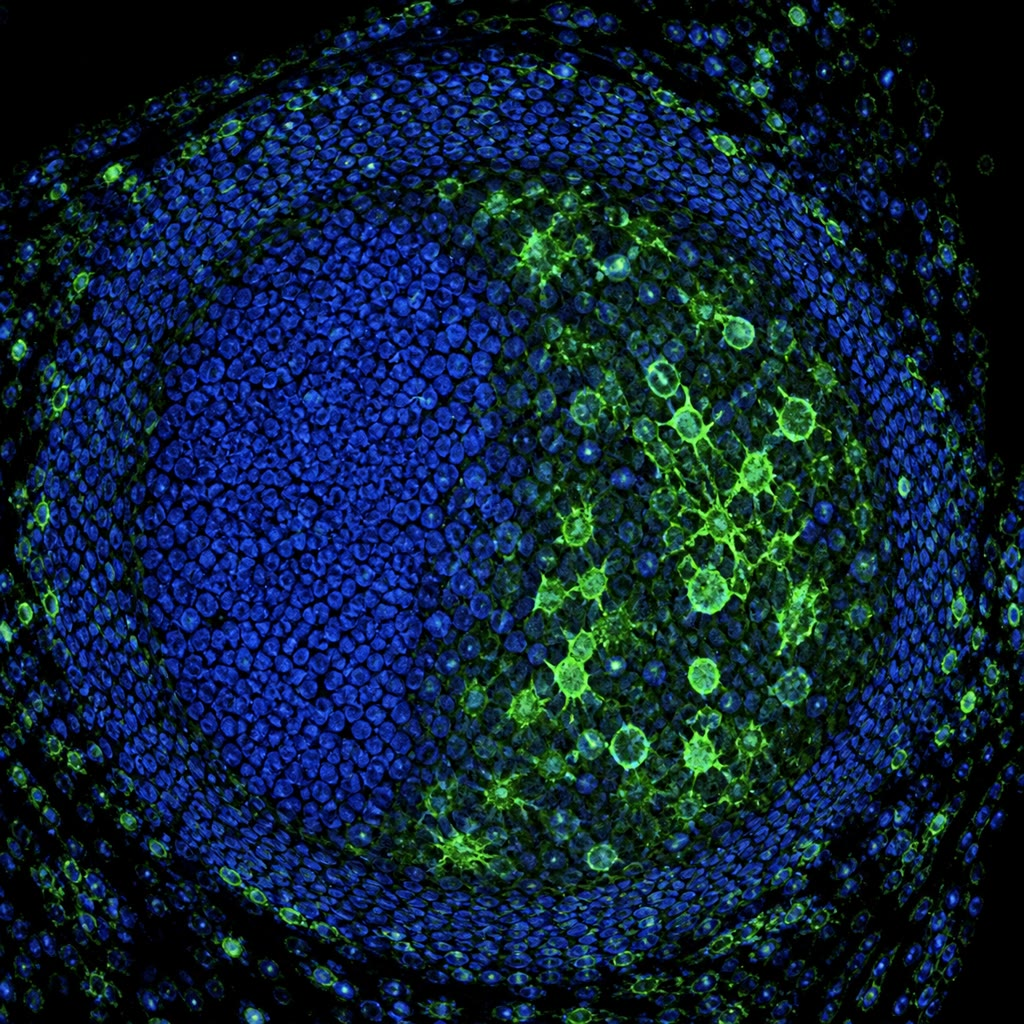
\includegraphics[width=0.36\linewidth]{images/book5/ai/b5-16-germinal-centre.jpg}\hspace{0.04\linewidth}
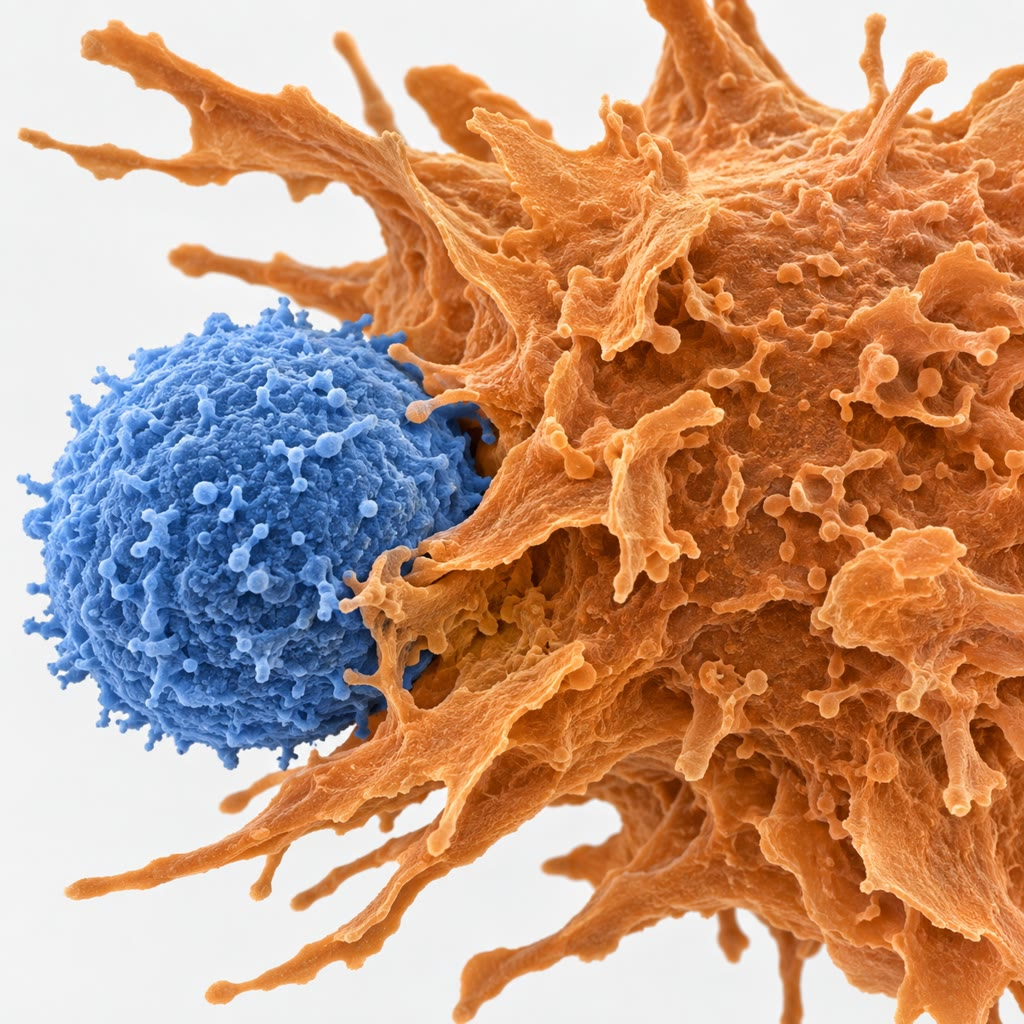
\includegraphics[width=0.36\linewidth]{images/book5/ai/b5-16-t-cell-apc.jpg}

{\small À esquerda: um \omterm{def:b3:adaptive-immunity:germinal-centre}{centro germinativo} num \omterm{def:b3:adaptive-immunity:lymphocytes}{linfonodo} --- a zona
escura apinhada e a zona mais clara da seleção. À direita: uma \omterm{def:b3:adaptive-immunity:lymphocytes}{célula T}
(pequena) em contato com uma \omterm{def:b3:innate-immunity:innate}{célula dendrítica}, o momento em que a
resposta adaptativa é decidida.}
\end{omfigure}

\section{A tolerância e suas falhas}

\begin{definition}[Tolerância]\label{def:b3:adaptive-immunity:tolerance}
\index{tolerância}\index{seleção negativa}\index{timo}\index{anergia}\index{FoxP3}\index{autoimunidade}
O repertório é feito ao acaso e contém, portanto, receptores para o
próprio. A \emph{tolerância central} os remove no lugar onde as células
amadurecem: no timo, as \omterm{def:b3:adaptive-immunity:lymphocytes}{células T} cujos receptores ligam peptídeo--MHC
próprio com força demais são mortas (\emph{seleção negativa}), as que
não conseguem ligar MHC nenhum também são mortas (seriam inúteis), e só
os poucos por cento intermediários saem; um fator de transcrição, o
AIRE, faz as células tímicas expressarem proteínas de todos os tecidos
--- insulina, tireoglobulina --- para que as \omterm{def:b3:adaptive-immunity:lymphocytes}{células T} específicas para
elas possam ser deletadas ali. As \omterm{def:b3:adaptive-immunity:lymphocytes}{células B} que ligam o próprio na
medula são deletadas ou editam seus receptores. A \emph{tolerância
periférica} cuida do resto: uma \omterm{def:b3:adaptive-immunity:lymphocytes}{célula T} que encontra seu \omterm{def:b3:adaptive-immunity:lymphocytes}{antígeno} sem
\omterm{def:b3:adaptive-immunity:response}{coestimulação} é tornada não responsiva (\emph{anergia}) ou deletada; e
as \omterm{def:b3:adaptive-immunity:lymphocytes}{células T} \emph{reguladoras}, definidas pelo fator FoxP3, suprimem
ativamente as respostas contra o próprio e contra \omterm{def:b3:adaptive-immunity:lymphocytes}{antígenos} inofensivos
como os alimentos e os comensais. A \emph{autoimunidade} é a falha
desses controles: o diabetes tipo~1 (as \omterm{def:b3:adaptive-immunity:lymphocytes}{células T} destroem as células
$\beta$), a esclerose múltipla (a mielina), a artrite reumatoide (as
articulações), o lúpus (\omterm{def:b3:adaptive-immunity:antibody}{anticorpos} contra componentes nucleares), as
doenças da tireoide; cada uma se associa a alelos \omterm{def:b3:adaptive-immunity:mhc}{HLA} específicos, que
apresentam os peptídeos próprios relevantes, e algumas são disparadas
pela infecção por um micróbio cujos peptídeos se parecem com uma
proteína própria (a febre reumática após infecção estreptocócica).
\end{definition}

\begin{proof}[Evidência]
Medawar (1953) injetou células de uma linhagem consanguínea de
camundongos em camundongos recém-nascidos de outra; adultos, os
receptores aceitaram enxertos de pele da linhagem doadora que de outro
modo teriam rejeitado, ao mesmo tempo que rejeitavam enxertos de
terceiras linhagens. A \omterm{def:b3:adaptive-immunity:tolerance}{tolerância} era adquirida, específica e fixada
pelo que o sistema imune encontrou cedo --- a base experimental da
deleção dos clones autorreativos de Burnet. As crianças que nascem sem
um gene AIRE funcional desenvolvem \omterm{def:b3:adaptive-immunity:tolerance}{autoimunidade} contra muitos órgãos ao
mesmo tempo; as que não têm \omterm{def:b3:adaptive-immunity:tolerance}{FoxP3} (uma síndrome rara ligada ao X)
desenvolvem \omterm{def:b3:adaptive-immunity:tolerance}{autoimunidade} fatal na primeira infância --- os dois braços
da \omterm{def:b3:adaptive-immunity:tolerance}{tolerância}, cada um revelado por sua ausência.
\end{proof}

\begin{example}[Hipersensibilidade, deficiência, transplante]\label{ex:b3:adaptive-immunity:failures}
A \emph{alergia} é uma resposta Th2 a um \omterm{def:b3:adaptive-immunity:lymphocytes}{antígeno} inofensivo --- pólen,
amendoim, penicilina --- que produz IgE; na reexposição o \omterm{def:b3:adaptive-immunity:lymphocytes}{antígeno} faz
ligação cruzada da IgE nos mastócitos, que liberam histamina em minutos,
e, se o \omterm{def:b3:adaptive-immunity:lymphocytes}{antígeno} está no sangue, a liberação sistêmica é a
\emph{anafilaxia}, tratada com adrenalina. \emph{Imunodeficiência}: as
crianças sem \omterm{def:b3:adaptive-immunity:antibody}{RAG} ou sem a enzima ADA não fazem \omterm{def:b3:adaptive-immunity:lymphocytes}{linfócitos}
(imunodeficiência combinada grave) e morrem de infecção se não
receberem medula ou terapia gênica; o HIV destrói as \omterm{def:b3:adaptive-immunity:lymphocytes}{células T} CD4 e,
com elas, a ajuda de que toda resposta precisa. \emph{Transplante}: as
\omterm{def:b3:adaptive-immunity:lymphocytes}{células T} do receptor veem as moléculas de \omterm{def:b3:adaptive-immunity:mhc}{HLA} do doador como estranhas,
e até um décimo de todas as \omterm{def:b3:adaptive-immunity:lymphocytes}{células T} responde --- muito mais do que a
qualquer patógeno ---, de modo que os enxertos são pareados nos loci do
\omterm{def:b3:adaptive-immunity:mhc}{HLA} e o receptor fica imunossuprimido a vida toda; um enxerto de medula
pode, ao contrário, atacar seu novo hospedeiro. E os usos deliberados:
os \omterm{def:b3:adaptive-immunity:antibody}{anticorpos} monoclonais do \cref{ch:b3:genetic-engineering}, os
inibidores de checkpoint que soltam as \omterm{def:b3:adaptive-immunity:lymphocytes}{células T} contra os \omterm{def:b3:cancer-biology:hallmarks}{tumores}
(\cref{ch:b3:cancer-biology}) e as \omterm{def:b3:adaptive-immunity:lymphocytes}{células T} modificadas com um receptor
quimérico para um \omterm{def:b3:adaptive-immunity:lymphocytes}{antígeno} tumoral (CAR-T), que curaram leucemias que
nada mais alcançava.
\end{example}

\section{Vacinação}

\begin{definition}[Vacinas e imunidade coletiva]\label{def:b3:adaptive-immunity:vaccine}
\index{vacina}\index{imunidade coletiva}\index{número básico de reprodução}\index{eficácia vacinal}
Uma \emph{vacina} apresenta \omterm{def:b3:adaptive-immunity:lymphocytes}{antígenos} de um patógeno, com um adjuvante
ou numa forma que dispara os receptores inatos, para que quem a recebe
adquira \omterm{def:b3:adaptive-immunity:response}{células de memória} e \omterm{def:b3:adaptive-immunity:antibody}{anticorpos} sem a doença (o
\cref{ch:b3:virology} lista os tipos). Sua \emph{eficácia} $E$ é a
fração de pessoas vacinadas que ficam protegidas. A proteção vai além
dos vacinados: um patógeno que se espalha numa população em que cada
caso infecta em média $R_{0}$ outros quando todos são suscetíveis --- o
\emph{número básico de reprodução} --- infecta apenas $R_{0}$ vezes a
fração suscetível quando alguns são imunes, e se extingue quando esse
número cai abaixo de um. É a \emph{imunidade coletiva}: acima de um
limiar de pessoas imunes a cadeia de transmissão se rompe e os não
vacinados --- lactentes, imunocomprometidos, aqueles em quem a vacina
falhou --- ficam protegidos pelos demais.
\end{definition}

\begin{theorem}[O limiar de imunidade coletiva]\label{thm:b3:adaptive-immunity:herd}
\index{imunidade coletiva!limiar}\index{modelo SIR}
Numa população em que uma fração $p$ é imune e o restante é suscetível,
cada caso infecta em média $R_{\text{eff}} = R_{0}(1 -
p)$ outros. Uma
epidemia não pode começar se $R_{\text{eff}} < 1$, isto é, se
\[
p > p_{c} = 1 - \frac{1}{R_{0}} .
\]
Com uma \omterm{def:b3:adaptive-immunity:vaccine}{vacina} de eficácia $E$, a cobertura necessária é $f_{c} = p_{c}/E$. Se uma epidemia de fato corre numa população suscetível (o
\omterm{thm:b3:adaptive-immunity:herd}{modelo SIR}, com taxa de infecção $\beta$ e taxa de recuperação $\gamma$,
$R_{0} =
\beta/\gamma$), ela atinge o pico quando a fração suscetível
cai a $1/R_{0}$, e a fração jamais infectada, $s_{\infty}$, satisfaz
$\ln s_{\infty} = -R_{0}(1 - s_{\infty})$.
\end{theorem}
\begin{proof}
Cada caso faz contatos que infectariam $R_{0}$ pessoas se todas fossem
suscetíveis; uma fração $1 - p$ delas é, de modo que $R_{\text{eff}} =
R_{0}(1-p)$, e a condição $R_{\text{eff}} < 1$ dá $p_{c}$; uma \omterm{def:b3:adaptive-immunity:vaccine}{vacina} que
protege uma fração $E$ dos que a recebem torna imune uma fração $Ef$ da
população, de modo que $Ef > p_{c}$. No \omterm{thm:b3:adaptive-immunity:herd}{modelo SIR},
$\mathrm{d}s/\mathrm{d}t = -\beta si$ e $\mathrm{d}i/\mathrm{d}t =
\beta si - \gamma i = \gamma i(R_{0}s - 1)$, de modo que $i$ cresce
enquanto $s >
1/R_{0}$ e cai depois: o pico está em $s = 1/R_{0}$.
Dividindo as duas equações, $\mathrm{d}i/\mathrm{d}s = -1 + 1/(R_{0}s)$,
de modo que $i + s -
\ln s/R_{0}$ é constante; avaliando-a no início
($s = 1$, $i
\approx 0$) e no fim ($i = 0$, $s = s_{\infty}$) obtém-se
$s_{\infty} - \ln s_{\infty}/R_{0} = 1$, a relação de tamanho final.
\end{proof}

\begin{example}[Sarampo e varíola]\label{ex:b3:adaptive-immunity:measles}
O sarampo tem $R_{0} \approx 15$: $p_{c} = 1 - 1/15 = 93\,\%$ e, com uma
\omterm{def:b3:adaptive-immunity:vaccine}{vacina} de eficácia $97\,\%$ após duas doses, a cobertura necessária é de
$96\,\%$ --- razão pela qual o sarampo volta onde quer que a vacinação
escorregue alguns por cento, e pela qual uma criança não vacinada num
país bem vacinado está, ainda assim, segura. A varíola tinha $R_{0} \approx 5$--$7$, um limiar perto de $80$--$85\,\%$, nenhum reservatório
animal, nenhum portador assintomático e uma \omterm{def:b3:adaptive-immunity:vaccine}{vacina} que funcionava em
uma dose: erradicável, e erradicada. A poliomielite está quase lá. A
gripe e os coronavírus, cujos \omterm{def:b3:adaptive-immunity:lymphocytes}{antígenos} derivam (\cref{ch:b3:virology})
e cuja imunidade se desgasta, não estão. Numa população não vacinada uma
epidemia com $R_{0} = 3$ infecta, pela relação de tamanho final, $1 - s_{\infty} = 94\,\%$ das pessoas; com $R_{0} = 1.5$, $58\,\%$.
\end{example}

\begin{omfigure}
\begin{tikzpicture}
\begin{axis}[
  width=6.4cm, height=5.4cm,
  axis x line=bottom, axis y line=left,
  xmin=1, xmax=18, ymin=0, ymax=1,
  xlabel={$R_{0}$}, ylabel={limiar $p_{c}$},
  xlabel style={font=\small, at={(axis description cs:0.5,-0.12)}, anchor=north}, ylabel style={font=\small},
  tick label style={font=\scriptsize}, xtick={1,3,6,9,12,15,18}, ytick={0,0.5,0.8,0.93,1}, yticklabels={0,0.5,0.8,0.93,1},
  clip=false,
]
\addplot[very thick, omDef, domain=1:18, samples=80] {1-1/x};
\fill[omThm] (axis cs:15,0.933) circle (2pt); \node[font=\scriptsize, anchor=south east] at (axis cs:15,0.94) {sarampo};
\fill[omThm] (axis cs:6,0.833) circle (2pt); \node[font=\scriptsize, anchor=north west] at (axis cs:6.3,0.82) {varíola};
\fill[omThm] (axis cs:2.5,0.6) circle (2pt); \node[font=\scriptsize, anchor=north west] at (axis cs:2.6,0.58) {gripe de 1918};
\end{axis}
\begin{axis}[
  at={(7.6cm,0)}, anchor=south west,
  width=6.4cm, height=5.4cm,
  axis x line=bottom, axis y line=left,
  xmin=0, xmax=60, ymin=0, ymax=0.35,
  xlabel={dias}, ylabel={fração infecciosa},
  xlabel style={font=\small, at={(axis description cs:0.5,-0.12)}, anchor=north}, ylabel style={font=\small},
  tick label style={font=\scriptsize}, xtick={0,20,40,60}, ytick={0,0.1,0.2,0.3},
  clip=false,
]
\addplot[very thick, omThm, smooth] coordinates {(0,0.001) (5,0.003) (10,0.012) (15,0.04) (20,0.12) (25,0.25) (28,0.30) (31,0.27) (35,0.18) (40,0.09) (45,0.04) (50,0.015) (55,0.006) (60,0.002)};
\addplot[very thick, omDef, smooth] coordinates {(0,0.001) (5,0.0015) (10,0.0025) (15,0.004) (20,0.006) (25,0.009) (30,0.012) (35,0.014) (40,0.015) (45,0.014) (50,0.012) (55,0.009) (60,0.007)};
\node[font=\scriptsize, omThm, anchor=west] at (axis cs:30,0.3) {sem imunidade, $R_{0} = 3$};
\node[font=\scriptsize, omDef, anchor=south west] at (axis cs:32,0.03) {\qty{60}{\%} vacinados: $R_{\text{eff}} = 1.2$};
\end{axis}
\end{tikzpicture}

{\small À esquerda: o limiar $1 - 1/R_{0}$ --- quanto mais contagiosa a
doença, mais perto de todo mundo tem de estar imune. À direita: uma
epidemia SIR com $R_{0} = 3$ numa população virgem e numa com
\qty{60}{\%} de imunes, o que não basta para detê-la mas a achata e a
retarda.}
\end{omfigure}

\begin{omfigure}
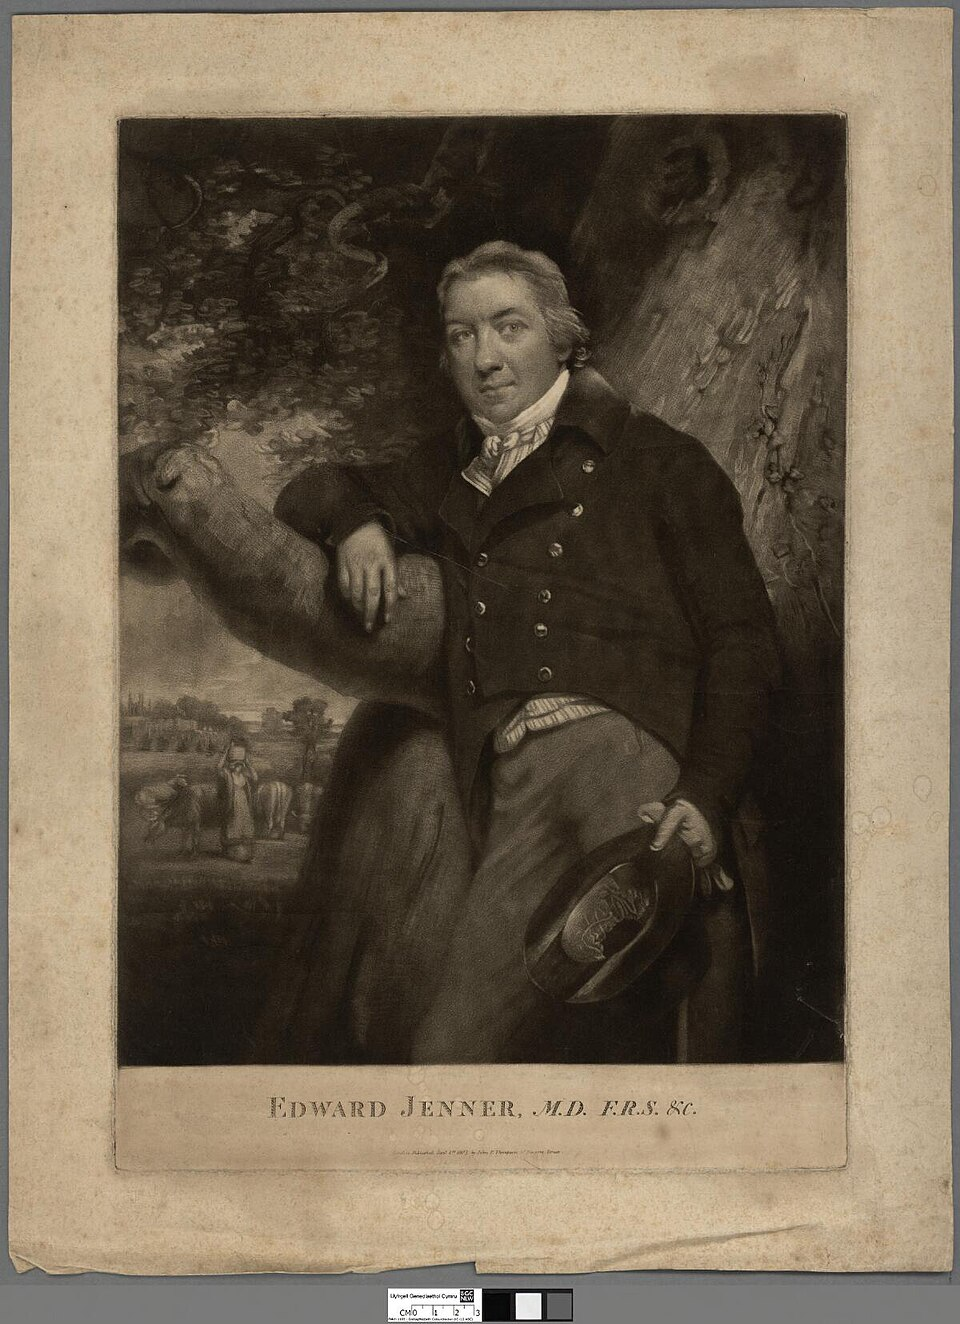
\includegraphics[width=0.30\linewidth]{images/book5/jenner.jpg}\hspace{0.04\linewidth}
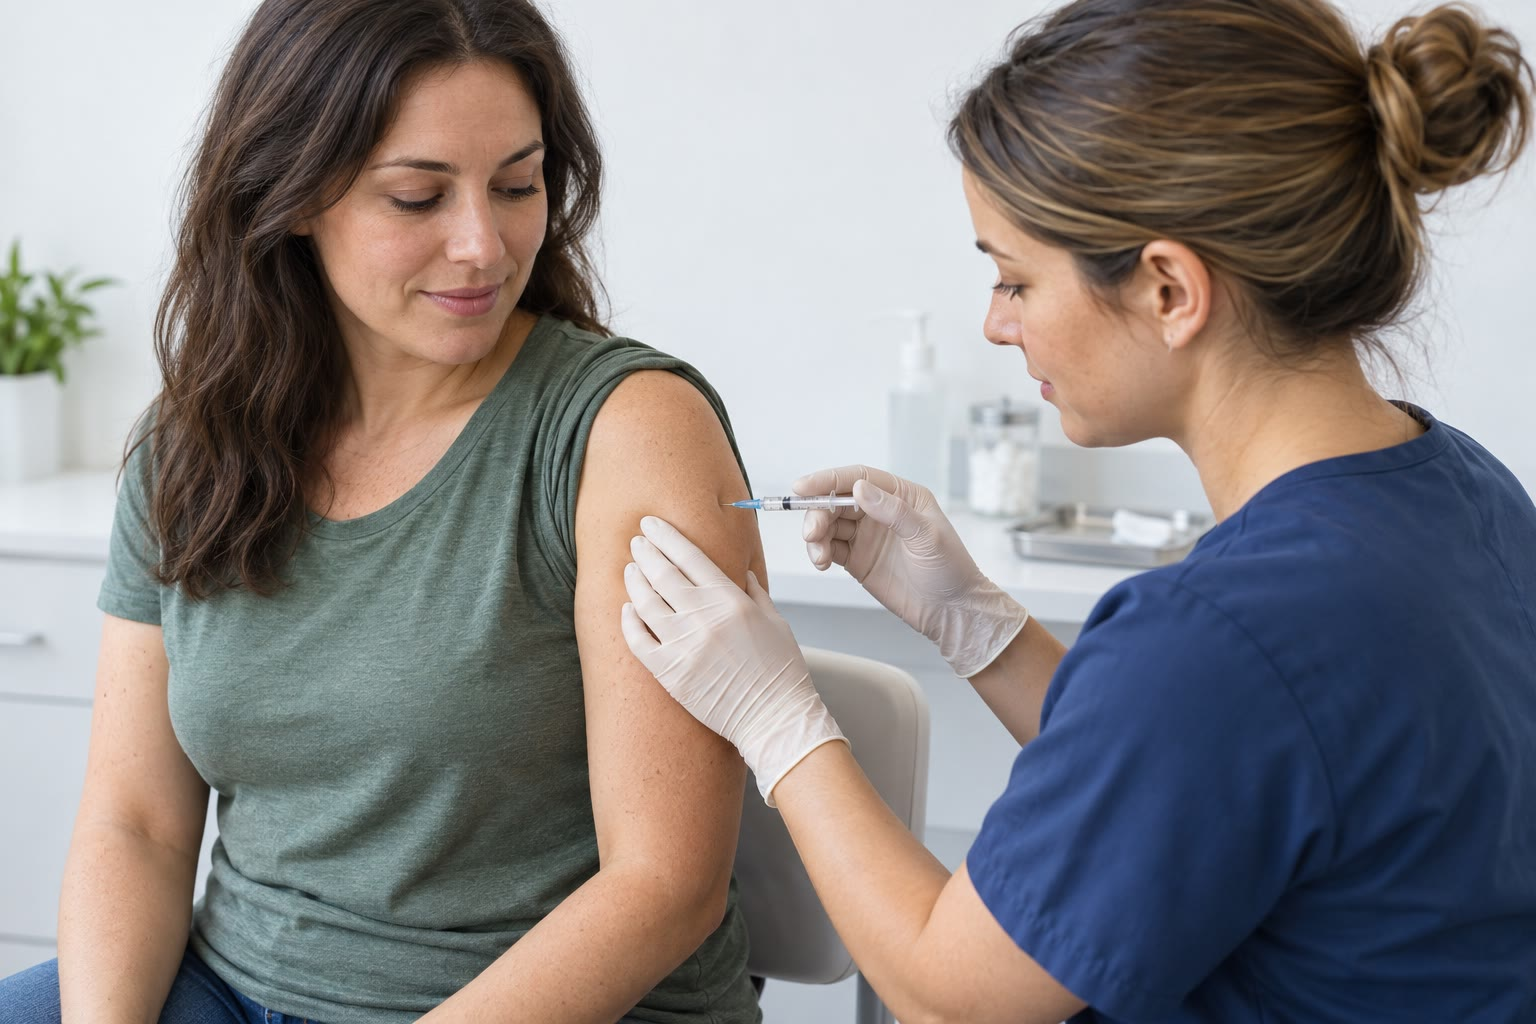
\includegraphics[width=0.50\linewidth]{images/book5/ai/b5-16-vaccination.jpg}

{\small Edward Jenner, que em 1796 protegeu um menino contra a varíola
com varíola bovina e fundou a vacinação (gravura de 1807, domínio
público). À direita: o mesmo ato dois séculos depois --- uma \omterm{def:b3:adaptive-immunity:vaccine}{vacina}
intramuscular, cujo \omterm{def:b3:adaptive-immunity:lymphocytes}{antígeno} as \omterm{def:b3:innate-immunity:innate}{células dendríticas} do deltoide levarão
aos \omterm{def:b3:adaptive-immunity:lymphocytes}{linfonodos} axilares.}
\end{omfigure}

\begin{remark}[O que a imunidade lembra]\label{rem:b3:adaptive-immunity:memory}
O sistema imune adaptativo é uma máquina darwiniana dentro de cada um de
nós: variação ao acaso (V(D)J, hipermutação), seleção (pelo \omterm{def:b3:adaptive-immunity:lymphocytes}{antígeno}, no
\omterm{def:b3:adaptive-immunity:germinal-centre}{centro germinativo}, contra o próprio no \omterm{def:b3:adaptive-immunity:tolerance}{timo}) e herança (\omterm{def:b3:adaptive-immunity:response}{células de
memória}, expansão clonal). Ele resolve, em semanas, o problema que a
evolução resolve em milênios --- uma molécula que liga um alvo nunca
visto antes --- e suas respostas estão entre os casos mais bem
estudados de evolução observada diretamente. Seu custo é a
\omterm{def:b3:adaptive-immunity:tolerance}{autoimunidade}, sua dependência do julgamento do sistema inato é
absoluta, e sua memória, que Jenner explorou e que as \omterm{def:b3:adaptive-immunity:vaccine}{vacinas} escrevem
de propósito, é a razão pela qual uma espécie de animais longevos e de
reprodução lenta pode sobreviver num mundo de micróbios de reprodução
rápida.
\end{remark}

\section{Exercícios}

\begin{exercise}[$\star$]\label{exo:b3:adaptive-immunity:1}
Enuncie os quatro princípios da \omterm{def:b3:adaptive-immunity:lymphocytes}{seleção clonal} e o experimento que
sustenta cada um dos dois primeiros.
\end{exercise}

\begin{exercise}[$\star$]\label{exo:b3:adaptive-immunity:2}
Descreva a estrutura de um \omterm{def:b3:adaptive-immunity:antibody}{anticorpo} e dê a função de cada uma das
cinco classes.
\end{exercise}

\begin{exercise}[$\star$]\label{exo:b3:adaptive-immunity:3}
Contraste o \omterm{def:b3:adaptive-immunity:mhc}{MHC de classe~I} e o de classe~II quanto à distribuição
celular, à origem do peptídeo, ao comprimento do peptídeo e à \omterm{def:b3:adaptive-immunity:lymphocytes}{célula T}
que lê cada um.
\end{exercise}

\begin{exercise}[$\star$]\label{exo:b3:adaptive-immunity:4}
Defina $R_{0}$ e o limiar de \omterm{def:b3:adaptive-immunity:vaccine}{imunidade coletiva}, e calcule o limiar
para a caxumba ($R_{0} = 5$), a coqueluche ($R_{0} = 12$) e a gripe de
1918 ($R_{0} = 2.5$).
\end{exercise}

\begin{exercise}[$\star\star$]\label{exo:b3:adaptive-immunity:5}
Uma espécie tem $V_{H} = 50$, $D = 20$, $J_{H} = 5$ e um único lócus
leve com $V = 60$, $J = 4$. Calcule o repertório combinatório e, em
seguida, o total com um fator juncional de $10^{4}$. Como ele se compara
com as $10^{9}$ \omterm{def:b3:adaptive-immunity:lymphocytes}{células B} que o animal tem?
\end{exercise}

\begin{exercise}[$\star\star$]\label{exo:b3:adaptive-immunity:6}
A região variável de uma \omterm{def:b3:adaptive-immunity:lymphocytes}{célula B} de \omterm{def:b3:adaptive-immunity:germinal-centre}{centro germinativo} tem
\qty{1000}{bp}; a AID muta a $10^{-3}$ por par de bases por divisão. Ao
longo de $20$ divisões, quantas mutações por célula e, entre $10^{5}$
células, quantas variantes distintas de base única do \omterm{def:b3:adaptive-immunity:antibody}{anticorpo} são
geradas? Compare com as $3000$ substituições únicas possíveis.
\end{exercise}

\begin{exercise}[$\star\star$]\label{exo:b3:adaptive-immunity:7}
Explique por que uma \omterm{def:b3:adaptive-immunity:lymphocytes}{célula T} de uma pessoa não reconhece peptídeos
virais apresentados pelas células de outra pessoa, e por que esse mesmo
fato torna difíceis os transplantes e polimórfico o sistema \omterm{def:b3:adaptive-immunity:mhc}{HLA}.
\end{exercise}

\begin{exercise}[$\star\star$]\label{exo:b3:adaptive-immunity:8}
Preveja o fenótipo imunológico de uma criança sem (a) RAG1, (b) AIRE,
(c) \omterm{def:b3:adaptive-immunity:tolerance}{FoxP3}, (d) a enzima de \omterm{def:b3:adaptive-immunity:antibody}{troca de classe} AID e (e) \omterm{def:b3:adaptive-immunity:lymphocytes}{células T} CD4.
\end{exercise}

\begin{exercise}[$\star\star$]\label{exo:b3:adaptive-immunity:9}
Uma \omterm{def:b3:adaptive-immunity:vaccine}{vacina} tem eficácia de \qty{90}{\%} e a doença, $R_{0} = 6$. Que
cobertura interrompe a transmissão? Se a cobertura for de \qty{80}{\%},
quanto vale $R_{\text{eff}}$, e que fração da população uma epidemia
infecta (use a relação de tamanho final com $R_{0}$ substituído por
$R_{\text{eff}}$ entre os suscetíveis --- ou argumente por que isso está
aproximadamente certo)?
\end{exercise}

\begin{exercise}[$\star\star\star$]\label{exo:b3:adaptive-immunity:10}
Deduza a relação de tamanho final do teorema a partir das equações do
SIR e resolva-a numericamente para $R_{0} = 1.5$, $2$, $3$ e $5$. Por
que uma epidemia nunca infecta todo mundo, mesmo sem intervenção alguma?
\end{exercise}

\begin{exercise}[$\star\star\star$]\label{exo:b3:adaptive-immunity:11}
A \omterm{def:b3:adaptive-immunity:germinal-centre}{maturação de afinidade} eleva a ligação mil vezes em três semanas.
Trate o \omterm{def:b3:adaptive-immunity:germinal-centre}{centro germinativo} como uma população sob seleção: com uma taxa
de mutação de uma por célula por divisão, uma fração $10^{-2}$ das
mutações melhorando a afinidade por um fator $1.5$ e o restante neutro
ou prejudicial, quantas rodadas de seleção são necessárias para um ganho
de mil vezes, e quantas células cada rodada precisa triar? Comente por
que o \omterm{def:b3:adaptive-immunity:germinal-centre}{centro germinativo} é organizado em ciclos.
\end{exercise}

\begin{exercise}[$\star\star\star$]\label{exo:b3:adaptive-immunity:12}
As doenças autoimunes são mais comuns em mulheres e se associam a
alelos \omterm{def:b3:adaptive-immunity:mhc}{HLA}; o diabetes tipo~1 quintuplicou em cinquenta anos nos países
ricos. Proponha, com os mecanismos deste capítulo e do
\cref{ch:b3:microbiomes}, explicações para cada observação e um teste
para cada uma.
\end{exercise}

\section{Problema: Uma Campanha de Vacinação}

\begin{problem}[{Problema de fim de semana --- um repertório contado,
uma resposta cronometrada de cem células até um mililitro de soro, um
centro germinativo rodado como algoritmo evolutivo e uma campanha contra
o sarampo planejada em face do limiar coletivo, terminando no tamanho do
repertório, no anticorpo que um plasmócito faz num dia e na cobertura de
que um país precisa}]
\label{pb:b3:adaptive-immunity:1}
Dados: $V_{H} = 40$, $D = 25$, $J_{H} = 6$; loci leves $(40, 5)$ e
$(30, 4)$; fator juncional $3\times 10^{4}$. Um corpo tem $10^{11}$
\omterm{def:b3:adaptive-immunity:lymphocytes}{células B}; uma em $10^{5}$ liga um dado epítopo; $100$ precursores são
recrutados; divisão a cada \qty{8}{h} por $7$ dias; \qty{30}{\%} do
clone vira \omterm{def:b3:adaptive-immunity:response}{plasmócitos} que secretam $2000$ moléculas de IgG por segundo
cada um; a IgG tem \qty{150}{kDa}; volume plasmático de \qty{3}{L};
meia-vida da IgG de \qty{21}{d}. \omterm{def:b3:adaptive-immunity:germinal-centre}{Centro germinativo}: região variável de
\qty{1000}{bp}, $10^{-3}$ mutações por pb por divisão, uma em $100$
mutações melhora a afinidade por $1.5$. Sarampo: $R_{0} = 15$, \omterm{def:b3:adaptive-immunity:vaccine}{eficácia
vacinal} de $0.93$ após uma dose e de $0.97$ após duas; um país de
$5\times 10^{6}$ habitantes com $60\,000$ nascimentos por ano.

\medskip
\noindent\textbf{Parte I --- O repertório.}
\begin{enumerate}
  \item Calcule o repertório combinatório e o total com a \omterm{def:b3:adaptive-immunity:antibody}{diversidade
        juncional}.
  \item Compare com o número de \omterm{def:b3:adaptive-immunity:lymphocytes}{células B}. Que fração do repertório
        possível um corpo expressa de cada vez, e o que se segue disso
        para os repertórios de dois indivíduos?
  \item Quantas \omterm{def:b3:adaptive-immunity:lymphocytes}{células B} do corpo ligam o epítopo? Quantas, em média,
        num \omterm{def:b3:adaptive-immunity:lymphocytes}{linfonodo} que abriga $10^{8}$ \omterm{def:b3:adaptive-immunity:lymphocytes}{células B}?
  \item Um recém-nascido tem $10^{9}$ \omterm{def:b3:adaptive-immunity:lymphocytes}{células B}. Quantas ligam o
        epítopo, e por que a resposta de um recém-nascido é fraca mesmo
        assim?
  \item A terceira alça da cadeia pesada de um \omterm{def:b3:adaptive-immunity:antibody}{anticorpo} é feita pela
        \omterm{def:b3:adaptive-immunity:antibody}{diversidade juncional}. Explique por que essa alça é a parte mais
        variável da molécula e costuma ficar no centro do sítio de
        ligação.
  \item A \omterm{def:b3:adaptive-immunity:germinal-centre}{hipermutação somática} acrescenta diversidade depois da
        seleção; a V(D)J, antes. Por que é vantajoso ter as duas, nessa
        ordem?
\end{enumerate}

\medskip
\noindent\textbf{Parte II --- A resposta.}
\begin{enumerate}[resume]
  \item A partir de $100$ células que se dividem a cada \qty{8}{h},
        quantas há após $7$ dias? Quantos \omterm{def:b3:adaptive-immunity:response}{plasmócitos}?
  \item Quantas moléculas de IgG eles secretam por dia, e que massa?
        Que concentração sérica o produto de um dia dá em \qty{3}{L}?
  \item Depois de dez dias de secreção nessa taxa, ignorando o
        decaimento, qual é a concentração em g/L? Compare com a IgG
        total normal de \qty{10}{g/L}.
  \item Os \omterm{def:b3:adaptive-immunity:response}{plasmócitos} morrem após duas semanas; o \omterm{def:b3:adaptive-immunity:antibody}{anticorpo} então decai
        com meia-vida de \qty{21}{d}. Quanto tempo até a concentração da
        questão 9 cair cem vezes? O que mantém o \omterm{def:b3:adaptive-immunity:antibody}{anticorpo} por anos?
  \item Uma resposta secundária parte de $10^{5}$ \omterm{def:b3:adaptive-immunity:response}{células de memória}.
        Quantas células após $3$ dias, e como isso se compara com a
        resposta primária no dia 3 e no dia 7?
  \item Explique por que a IgM vem primeiro e a IgG depois numa resposta
        primária, e por que a resposta secundária é IgG desde o início.
\end{enumerate}

\medskip
\noindent\textbf{Parte III --- O \omterm{def:b3:adaptive-immunity:germinal-centre}{centro germinativo}.}
\begin{enumerate}[resume]
  \item Quantas mutações uma \omterm{def:b3:adaptive-immunity:lymphocytes}{célula B} adquire em sua região variável por
        divisão? E ao longo de $20$ divisões?
  \item Que fração das filhas de uma divisão carrega uma mutação que
        melhora? Num \omterm{def:b3:adaptive-immunity:germinal-centre}{centro germinativo} de $10^{4}$ células em divisão,
        quantas células melhoradas aparecem por divisão?
  \item Quantas melhorias sucessivas de $1.5$ dão um ganho de mil vezes
        em afinidade? Se cada rodada de seleção leva duas divisões
        (\qty{12}{h}), quanto tempo é isso?
  \item A maioria das mutações danifica o \omterm{def:b3:adaptive-immunity:antibody}{anticorpo}. Se \qty{50}{\%} das
        mutações destroem a ligação, que fração das células sobrevive à
        mutação de cada divisão, e por que a zona clara precisa matar a
        maioria das células?
  \item Uma \omterm{def:b3:adaptive-immunity:vaccine}{vacina} dada em duas doses com seis semanas de intervalo
        produz \omterm{def:b3:adaptive-immunity:antibody}{anticorpos} de afinidade mais alta que uma dose única.
        Explique com o \omterm{def:b3:adaptive-immunity:germinal-centre}{centro germinativo}.
  \item Alguns \omterm{def:b3:virology:virus}{vírus} (HIV, gripe) escapam dos \omterm{def:b3:adaptive-immunity:antibody}{anticorpos} mutando sua
        superfície. Explique por que o \omterm{def:b3:adaptive-immunity:germinal-centre}{centro germinativo} é, ainda
        assim, a base da esperança de uma \omterm{def:b3:adaptive-immunity:vaccine}{vacina} amplamente protetora.
\end{enumerate}

\medskip
\noindent\textbf{Parte IV --- A campanha.}
\begin{enumerate}[resume]
  \item Limiar coletivo para o sarampo e cobertura necessária com uma
        dose; com duas doses.
  \item O país \omterm{def:b3:adaptive-immunity:vaccine}{vacina} \qty{90}{\%} das crianças com duas doses. Fração
        imune, $R_{\text{eff}}$ e o veredito: o sarampo circula?
  \item Quantas crianças suscetíveis se acumulam por ano de nascimentos
        com cobertura de \qty{90}{\%} (não vacinadas mais falhas
        vacinais)? Depois de cinco anos sem sarampo, quantos suscetíveis
        existem, e por que uma importação causa então um surto?
  \item Use a relação de tamanho final com o número efetivo de
        reprodução entre os suscetíveis para estimar que fração desses
        suscetíveis um surto infecta. (Tome $R_{\text{eff}}$ da questão
        20 como o número de reprodução na população inteira, e note que
        dentro do grupo suscetível a doença se espalha como se $R_{0}$
        fosse $R_{\text{eff}}$.)
  \item A cobertura sobe para \qty{95}{\%} com duas doses. Fração imune
        e $R_{\text{eff}}$; o limiar é atingido?
  \item Lactentes com menos de um ano não podem ser vacinados contra o
        sarampo e são os mais propensos a morrer dele. Explique como a
        campanha os protege e o que acontece com essa proteção se a
        cobertura cair para \qty{85}{\%}.
  \item Resuma: o repertório total (questão~1), a IgG que os
        \omterm{def:b3:adaptive-immunity:response}{plasmócitos} de um dia fazem (questão~8) e a cobertura de duas
        doses de que o país precisa (questão~19).
\end{enumerate}
\end{problem}
